\documentclass[13pt,a4paper]{extarticle}
\usepackage[utf8]{inputenc}
\usepackage[utf8]{vietnam} %Bien dich duoc tieng Viet
\usepackage{amsmath,amsfonts,amssymb} %Font toan
\usepackage{type1cm}
\usepackage{times}
\usepackage{graphicx}
\graphicspath{ {images07/} }
\usepackage{enumerate}
\usepackage{comment}
\usepackage{multicol}
\usepackage{multirow}
%\usepackage[unicode]{hyperref} %Tu dong tao bookmark
\usepackage[unicode, hidelinks=true]{hyperref}
\usepackage{indentfirst} %Thut vao dau dong o tat ca cac doan
\usepackage{listings} %Dinh dang code
\usepackage{color} %Mau sac
\usepackage[left=2.5cm,right=2.5cm,top=2.5cm,bottom=2.5cm]{geometry} %Canh lề trái - phải - trên - dưới cho tài liệu
\usepackage{longtable}
\renewcommand{\arraystretch}{1.3}

\begin{document}
\pagenumbering{gobble}
\title{\Large{\textbf{BÀI CHUẨN BỊ THỰC TẬP ĐIỆN CÔNG NGHIỆP}}\\\vspace{1cm}\textbf{Bài 7}\\\vspace{.5cm}\textbf{MÔ HÌNH ĐIỀU KHIỂN NHIỆT ĐỘ BẰNG PHƯƠNG PHÁP ĐIỀU KHIỂN VÒNG KÍN PID THÔNG QUA BỘ BIẾN TẦN}}
\date{Ngày 14 tháng 06 năm 2016}
%\date{\today}
\author{GVHD: Võ Minh Thiện \vspace{.6cm}\\  Nhóm SVTH: Nhóm 2 -- Tiểu nhóm 1: Thi Minh Nhựt}
\maketitle
\tableofcontents
\newpage
\pagenumbering{arabic}
\setcounter{page}{1}
\section{Cơ sơ lý thuyết}
Bộ điều khiển vòng kín thực hiện so sánh giá trị đặt và giá trị đo được:
\begin{center}
\textit{Độ sai lệch = Giá trị đặt -- Giá trị đo}
\end{center}

Các trường hợp sau:
\begin{list}{+}{}
\item \textit{Nhiệt độ đo < Nhiệt độ cài đặt}: Bộ điều khiển sẽ tiếp tục đốt lò.
\item \textit{Nhiệt độ đo > Nhiệt độ cài đặt}: Bộ điều khiển sẽ giảm đốt và ngưng đốt lò.
\item[$\rightarrow$] Nhiệt độ lò được điều khiển quanh giá trị cài đặt.
\end{list}
\subsection{Điều khiển kiểu đóng ngắt}
Mô hình điều khiển như hình \ref{Fig:relay-nhiet-on-off}:
\begin{list}{--}{}
\item Sử dụng: relay nhiệt và khởi động từ.
\item Khi khởi động từ đóng: lò điện được cấp điện.
\item Khi khởi động từ ngắt: lò điện mất điện.
\item Relay nhiệt đóng: khi nhiệt độ thấp hơn nhiệt độ cài đặt.
\item Relay nhiệt ngắt: khi nhiệt độ cao hơn nhiệt độ cài đặt. 
\end{list}
\begin{figure}[!h]
\begin{center}
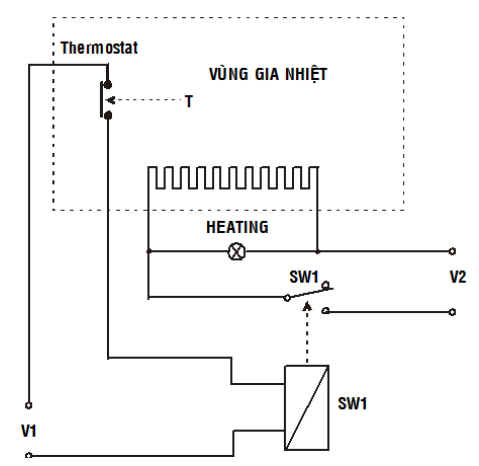
\includegraphics[scale=.6]{1}
\end{center}
\caption{Điều khiển kiểu đóng ngắt với Relay nhiệt}
\label{Fig:relay-nhiet-on-off}
\end{figure}
\subsection{Điều khiển kiểu tương tự}
Cho phép điều chỉnh liên tục quá trình đốt lò thông qua khóa điện tử:
\begin{list}{--}{}
\item Nếu nhiệt độ tiến gần nhiệt độ đặt: chu kỳ đốt lò thưa dần.
\item Nếu nhiệt độ chưa đủ nhiệt độ đặt: chu kỳ đốt lò ngắn.
\end{list}

Nguyên tắc điều khiển thuộc kiểu điểu khiển PID:
\begin{list}{--}{}
\item Tác động điều khiển tỷ lệ với sai lệch nhiệt độ $P$.
\item Tác động điều khiển liên tục khi có sai lệch nhiệt độ $I$.
\item Tác động điều khiển tỷ lệ với tốc độ sai lệch nhiệt độ $D$.
\end{list}
\section{Nội dung thực hành}
\subsection{Điều khiển kiểu ON/OFF cho nhiệt độ}
\subsubsection{Sơ đồ mạch}
\begin{figure}[!h]
\begin{center}
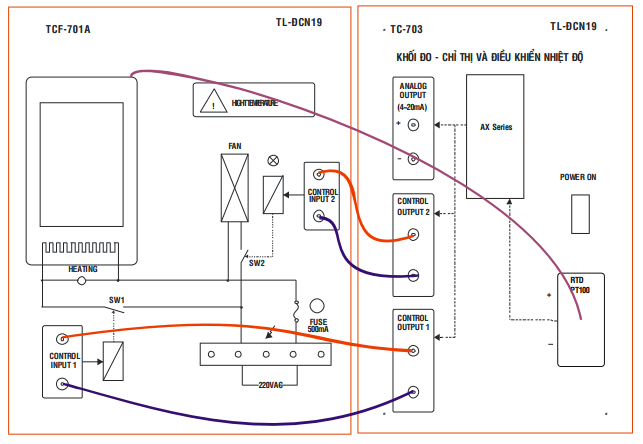
\includegraphics[scale=.6]{2}
\end{center}
\caption{Sơ đồ mạch điều khiển kiểu ON/OFF}
\label{Fig:mach-on-off}
\end{figure}
Mô tả sơ đồ:
\begin{list}{--}{}
\item Nối cảm biến nhiệt $RTD-PT100$ (gắn trên hốc lò) vào khối $RTD$ của khối đo và điều nhiệt.
\item Nối ngõ ra $Control~Output~1$ vào ngõ vào $Control~Input~1$: điều khiển đốt.
\item Nối ngõ ra $Control~Output~2$ vào ngõ vào $Control~Input~2$: điều khiển quạt làm mát.
\item Cấp nguồn $220VAC$ cho khối điều nhiệt $TCF-701A$.
\end{list}
\subsubsection{Thiết lập và điều khiển}
\begin{list}{--}{}
\item Thiết lập chế độ đo và điều khiển:
\begin{list}{+}{}
\item Cảm biến: \verb|Pt100|.
\item Chế độ điều khiển: \verb|ON/OFF|.
\item Kiểu tác động ra: nóng.
\item Lối ra: \verb|Relay 2/Control Output 1|.
\item Nhiệt độ đặt: $T= 100^0C$.
\item Chu kỳ điều khiển: $2s$.
\end{list}
\item Vận hành hệ thống nhiệt độ: Xác định $T_{max}$; $T_{min}$ (khi nhiệt độ đã ổn định).

Tính hệ số điều khiển nhiệt độ $\displaystyle K = \frac{T_{max}-T_{min}}{T_{tb}}$
\item Thiết lặp chu kỳ điều khiển bằng $20s$. Xác định $T_{max}$; $T_{min}$ (khi nhiệt độ đã ổn định).

Tính hệ số điều khiển nhiệt độ $\displaystyle K = \frac{T_{max}-T_{min}}{T_{tb}}$
\end{list}
\subsection{Điều khiển ON/OFF cho quạt làm mát}
\subsubsection{Sơ đồ mạch}
Sơ đồ mạch như hình \ref{Fig:mach-on-off} trang \pageref{Fig:mach-on-off}.
\subsubsection{Thiết lập và điều khiển}
\begin{list}{--}{}
\item Đặc giá trị nhiệt độ là $150^0C$.
\item Thiết lập chế độ điều khiển:
\begin{list}{+}{}
\item Chế độ điều khiển: \verb|ON/OFF|.
\item Lối ra: \verb|Relay 3/Control Output 2| cho làm mát.
\item Kiểu tác động ra: nóng.
\item Nhiệt độ đặc là $50^0C$.
\end{list}
\item Theo dõi nhiệt độ của quạt cho đến khi nhiệt độ giảm xuống giá trị đặt. Lấy các số liệu trên bộ điều khiển, xác định hệ số gia nhiệt.
\end{list}
\subsection{Điều khiển nhiệt độ tự động với bộ biến tần}
\subsubsection{Điều khiển kiểu ON/OFF}
\begin{list}{--}{}
\item Sơ đồ mạch như hình \ref{Fig:mach-on-off} trang \pageref{Fig:mach-on-off}.
\item Kết nối ngõ ra Output của bộ điều khiển nhiệt độ: đầu nối vào ngõ Run, Forward start của bộ biến tần.
\item Cấp nguồn động lực cho bộ biến tần, đấu nối biến tần và động cơ.
\item Cài đặt biến tần:
\begin{list}{+}{}
\item \verb|P0 = 03|: Moment trượt.
\item \verb|P1 = 50|: Tần số cực đại.
\item \verb|P2 = 0|: Tần số cực tiểu.
\item \verb|P3 = 50|: Tần số cơ bản.
\item \verb|P7 = 3|: Thời gian tăng tốc (giây).
\item \verb|P8 = 3|: Thời gian giảm tốc (giây).
\item \verb|P13 = 0|: Tần số khởi động. 
\item \verb|P79 = 0|: Vận hành bàn phím kết hợp với ngõ điều khiển.
\end{list}
\item Vận hành hệ thống: theo dõi nhiệt độ đến khi đạt giá trị đặt. Ghi nhận các giá trị hiển thị.
\item Xác lập lại chế độ đo và điều khiển: 
\begin{list}{+}{}
\item Chế độ điều khiển \verb|ON/OFF|.
\item Lối ra Relay 3/Control Output 2: cho quạt làm mát.
\item Tác động ra: nóng.
\item Nhiệt độ đặt $50^0C$.
\end{list}
\item Vận hành hệ thống: theo dõi nhiệt độ đến khi đạt giá trị đặt. Ghi nhận các giá trị hiển thị.
\end{list}
\subsubsection{Điều khiển nhiệt độ tự động theo phương pháp điều khiển vòng kín -- PID}
\begin{list}{--}{}
\item Sơ đồ mạch như hình \ref{Fig:mach-on-off} trang \pageref{Fig:mach-on-off}.
\item Kết nối ngõ ra Analog của bộ điều khiển nhiệt độ: đầu ngõ ra $4-20mA$ kết nối với ngõ số 4 và 5 của biến tần.
\item Cấp nguồn động lực cho bộ biến tần, đấu nối biến tần và động cơ.
\item Cài đặt biến tần:
\begin{list}{+}{}
\item \verb|P0 = 03|: Moment trượt.
\item \verb|P1 = 50|: Tần số cực đại.
\item \verb|P2 = 0|: Tần số cực tiểu.
\item \verb|P3 = 50|: Tần số cơ bản.
\item \verb|P7 = 3|: Thời gian tăng tốc (giây).
\item \verb|P8 = 3|: Thời gian giảm tốc (giây).
\item \verb|P13 = 0|: Tần số khởi động. 
\item \verb|P79 = 0|: Vận hành bàn phím kết hợp với ngõ điều khiển.
\end{list}
\item Cấu hình mở rộng: Chế độ điều khiển PID:
\begin{list}{+}{}
\item \verb|P160 = 0|: Thông số mở rộng.
\item \verb|P127 = 0-50|: PID tự động chuyển qua tần số.
\item \verb|P128 = 41|: Chọn lựa hoạt động PID.
\item \verb|P129 = 100|: Thông số hồi tiếp.
\item \verb|P130 = 2|: Thời gian hổi tiếp tín hiệu.
\item \verb|P131 = 100|: PID giới hạn trên.
\item \verb|P132 = 10|: PID giới hạn dưới.
\item \verb|P133 = 20|: Điểm hoạt động PID.
\item \verb|P134 = 1|: Thời gian đáp ứng giá trị hồi tiếp.
\end{list}
\item Vận hành hệ thống: theo dõi nhiệt độ đến khi đạt giá trị đặt. Ghi nhận các giá trị hiển thị.
\item Xác lập lại chế độ đo và điều khiển: 
\begin{list}{+}{}
\item Chế độ điều khiển \verb|ON/OFF|.
\item Lối ra Relay 3/Control Output 2: cho quạt làm mát.
\item Tác động ra: nóng.
\item Nhiệt độ đặt $50^0C$.
\end{list}
\item Vận hành hệ thống: theo dõi nhiệt độ đến khi đạt giá trị đặt. Ghi nhận các giá trị hiển thị.
\end{list}
\end{document}